\documentclass[11pt,a4paper]{report}
\usepackage[textwidth=37em,vmargin=30mm]{geometry}
\usepackage{calc,xunicode,amsmath,amssymb,paralist,enumitem,tabu,booktabs,datetime2,xeCJK,xeCJKfntef,listings}
\usepackage{tocloft,fancyhdr,tcolorbox,xcolor,graphicx,eso-pic,xltxtra,xelatexemoji}

\newcommand{\envyear}[0]{2025}
\newcommand{\envdatestr}[0]{2025-10-14}
\newcommand{\envfinaldir}[0]{webdb/2025/20251014/final}

\usepackage[hidelinks]{hyperref}
\hypersetup{
    colorlinks=false,
    pdfpagemode=FullScreen,
    pdftitle={Web Digest - \envdatestr}
}

\setlength{\cftbeforechapskip}{10pt}
\renewcommand{\cftchapfont}{\rmfamily\bfseries\large\raggedright}
\setlength{\cftbeforesecskip}{2pt}
\renewcommand{\cftsecfont}{\sffamily\small\raggedright}

\setdefaultleftmargin{2em}{2em}{1em}{1em}{1em}{1em}

\usepackage{xeCJK,xeCJKfntef}
\xeCJKsetup{PunctStyle=plain,RubberPunctSkip=false,CJKglue=\strut\hskip 0pt plus 0.1em minus 0.05em,CJKecglue=\strut\hskip 0.22em plus 0.2em}
\XeTeXlinebreaklocale "zh"
\XeTeXlinebreakskip = 0pt


\setmainfont{Brygada 1918}
\setromanfont{Brygada 1918}
\setsansfont{IBM Plex Sans}
\setmonofont{JetBrains Mono NL}
\setCJKmainfont{Noto Serif CJK SC}
\setCJKromanfont{Noto Serif CJK SC}
\setCJKsansfont{Noto Sans CJK SC}
\setCJKmonofont{Noto Sans CJK SC}

\setlength{\parindent}{0pt}
\setlength{\parskip}{8pt}
\linespread{1.15}

\lstset{
	basicstyle=\ttfamily\footnotesize,
	numbersep=5pt,
	backgroundcolor=\color{black!5},
	showspaces=false,
	showstringspaces=false,
	showtabs=false,
	tabsize=2,
	captionpos=b,
	breaklines=true,
	breakatwhitespace=true,
	breakautoindent=true,
	linewidth=\textwidth
}






\newcommand{\coverpic}[2]{
    % argv: itemurl, authorname
    Cover photo by #2~~(\href{#1}{#1})
}
\newcommand{\makeheader}[0]{
    \begin{titlepage}
        % \newgeometry{hmargin=15mm,tmargin=21mm,bmargin=12mm}
        \begin{center}
            
            \rmfamily\scshape
            \fontspec{BaskervilleF}
            \fontspec{Old Standard}
            \fontsize{59pt}{70pt}\selectfont
            WEB\hfill DIGEST
            
            \vfill
            % \vskip 30pt
            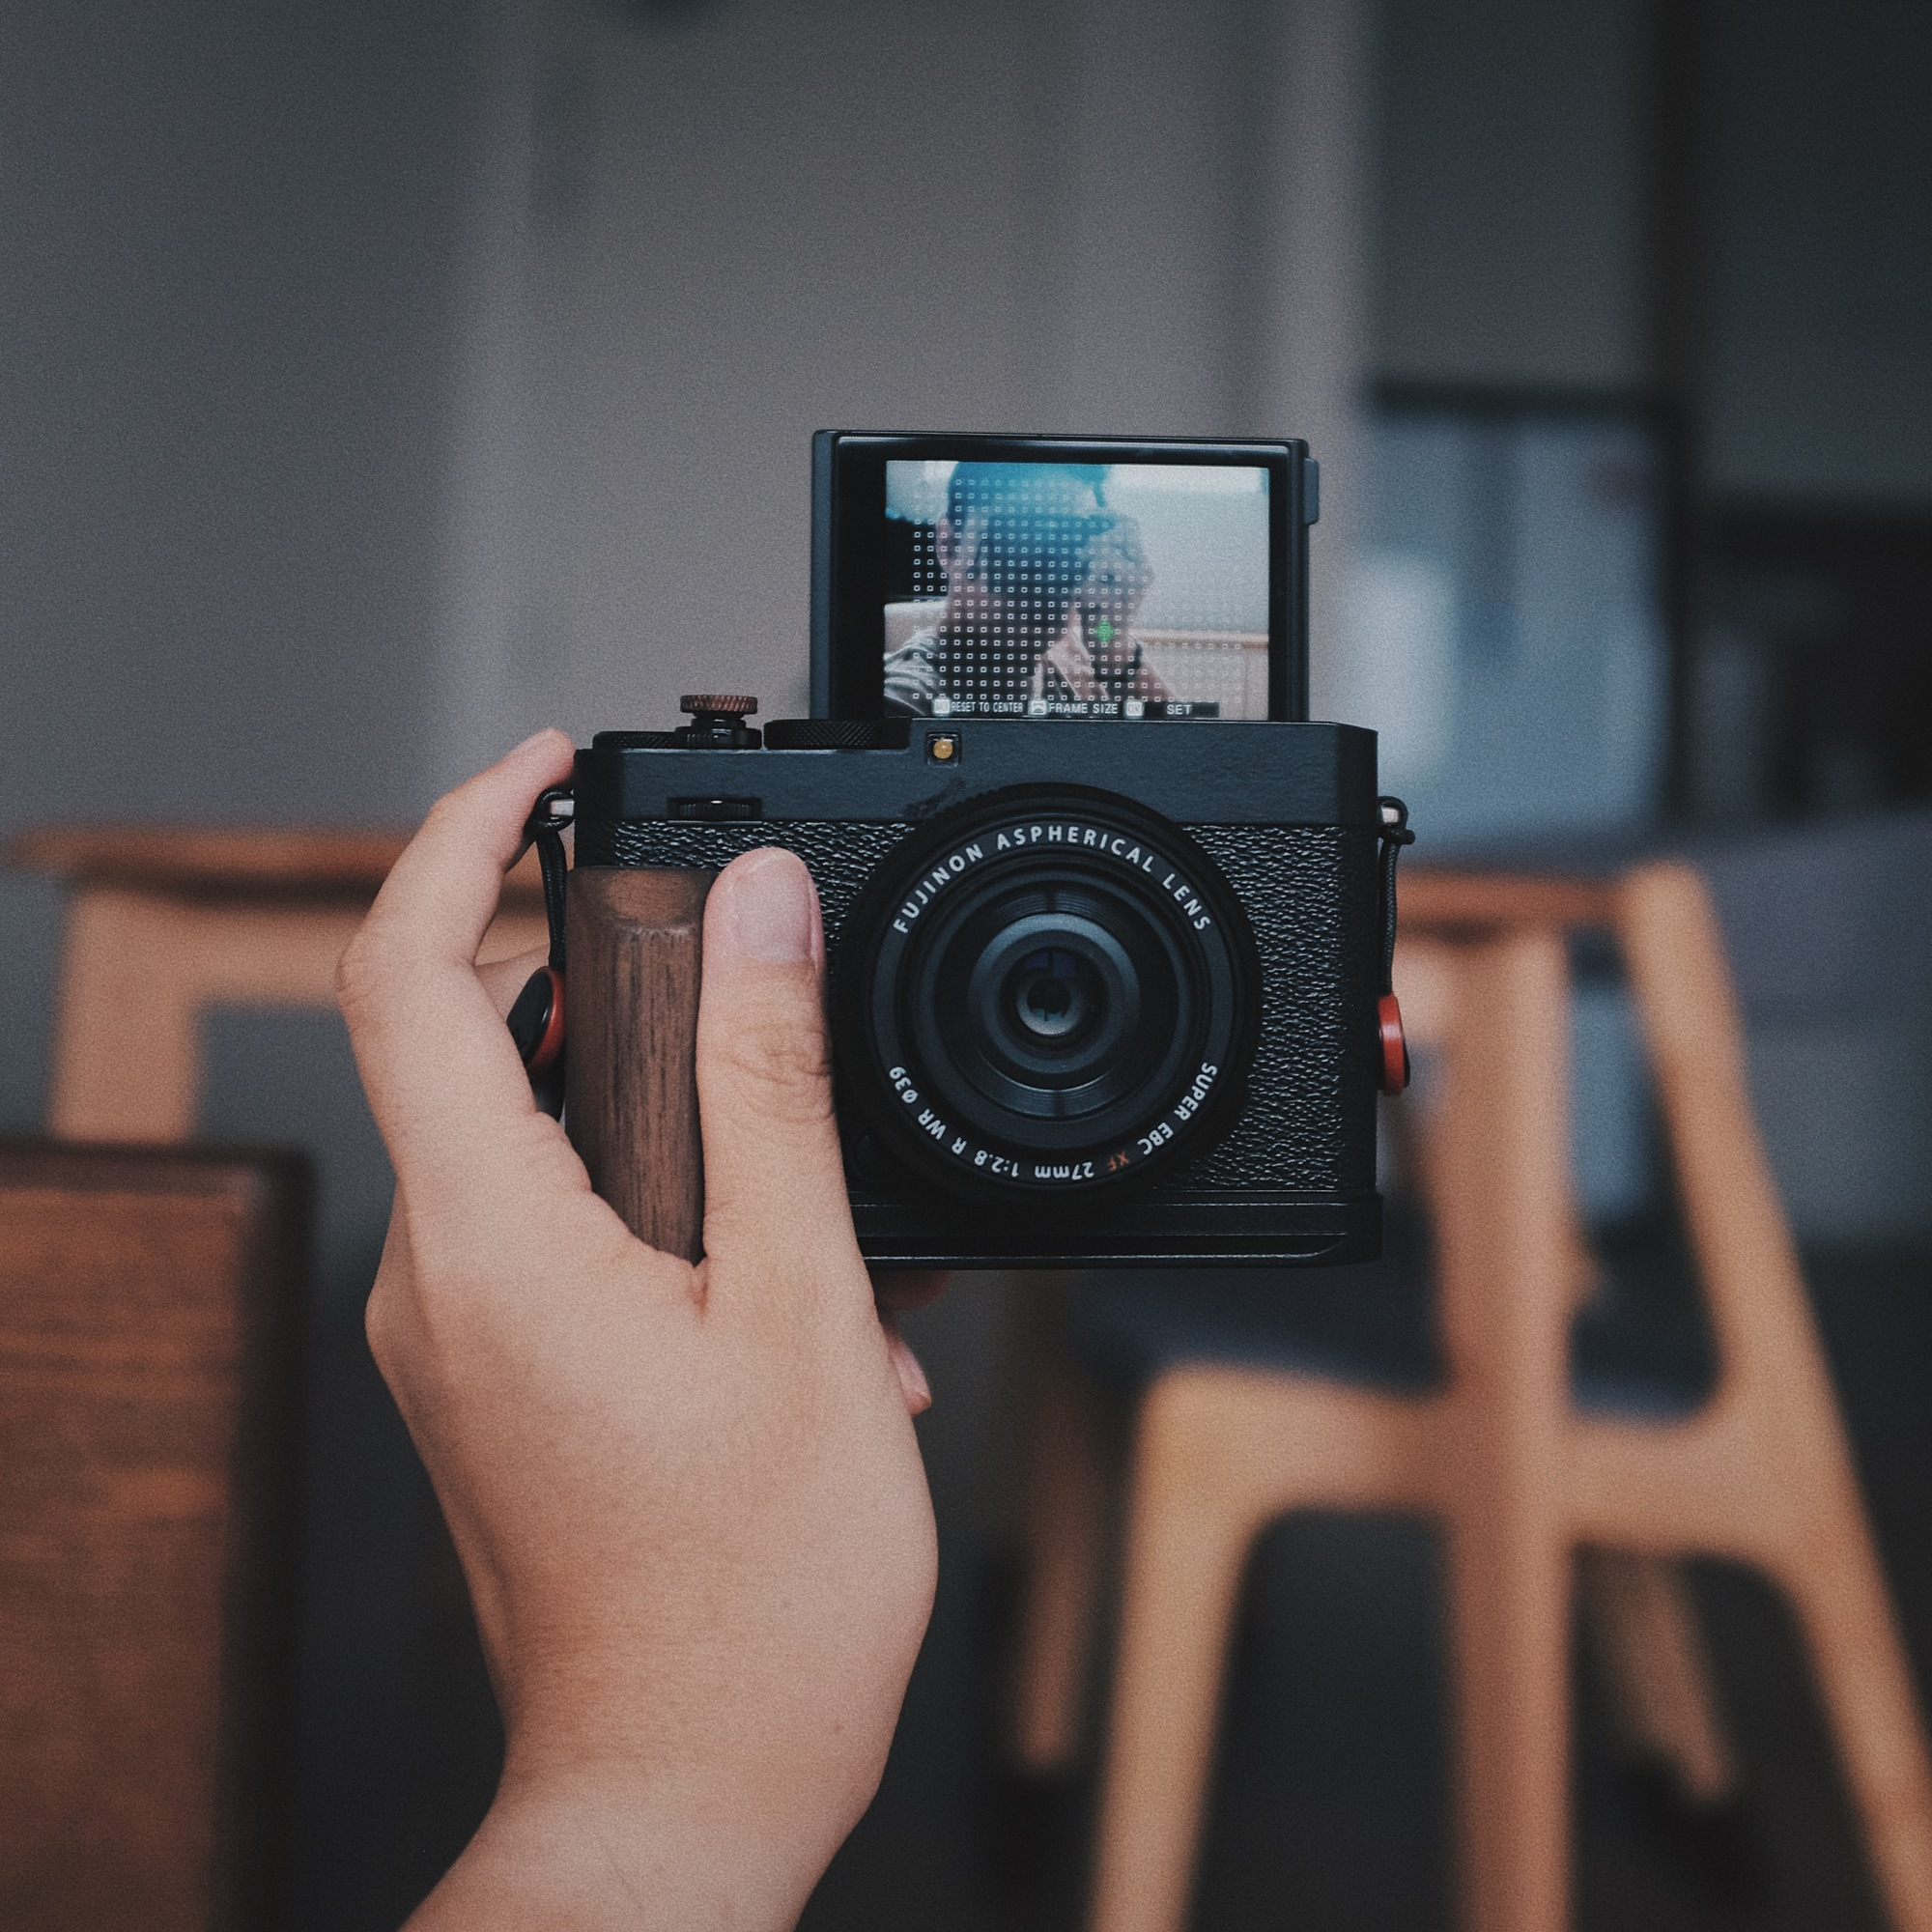
\includegraphics[width=\linewidth]{\envfinaldir/coverpic-prod.jpg}\par
            % \vskip 30pt
            \vfill

            \normalsize\rmfamily\scshape
            \copyright{} The Web Digest Project \hfill\large \envdatestr
        \end{center}
    \end{titlepage}
    % \restoregeometry
}
\newcommand{\simplehref}[1]{%
    \textcolor{blue!80!green}{\href{#1}{#1}}%
}
\renewcommand{\contentsname}{\center\Huge\sffamily\bfseries Contents\par\vskip 20pt}
\newcounter{ipartcounter}
\setcounter{ipartcounter}{0}
\newcommand{\ipart}[1]{
    % \vskip 20pt
    \clearpage
    \stepcounter{ipartcounter}
    \phantomsection
    \addcontentsline{toc}{chapter}{#1}
    % \begin{center}
    %     \Huge
    %     \sffamily\bfseries
    %     #1
    % \end{center}
    % \vskip 20pt plus 7pt
}
\newcounter{ichaptercounter}
\setcounter{ichaptercounter}{0}
\newcommand{\ichapter}[1]{
    % \vskip 20pt
    \clearpage
    \stepcounter{ichaptercounter}
    \phantomsection
    \addcontentsline{toc}{section}{\numberline{\arabic{ichaptercounter}}#1}
    \begin{center}
        \Huge
        \sffamily\bfseries
        #1
    \end{center}
    \vskip 20pt plus 7pt
}
\newcommand{\entrytitlefont}[1]{\subsection*{\raggedright\Large\sffamily\bfseries#1}}
\newcommand{\entryitemGeneric}[2]{
    % argv: title, url
    \parbox{\linewidth}{
        \entrytitlefont{#1}\par\vskip 5pt
        \footnotesize\ttfamily\mdseries
        \simplehref{#2}
    }\vskip 11pt plus 11pt minus 1pt
}
\newcommand{\entryitemGithub}[3]{
    % argv: title, url, desc
    \parbox{\linewidth}{
        \entrytitlefont{#1}\par\vskip 5pt
        \footnotesize\ttfamily\mdseries
        \simplehref{#2}\par\vskip 5pt
        \small\rmfamily\mdseries#3
    }\vskip 11pt plus 11pt minus 1pt
}
\newcommand{\entryitemAp}[3]{
    % argv: title, url, desc
    \parbox{\linewidth}{
        \entrytitlefont{#1}\par\vskip 5pt
        \footnotesize\ttfamily\mdseries
        \simplehref{#2}\par\vskip 5pt
        \small\rmfamily\mdseries#3
    }\vskip 11pt plus 11pt minus 1pt
}
\newcommand{\entryitemHackernews}[3]{
    % argv: title, hnurl, rawurl
    % \parbox{\linewidth}{
    %     \entrytitlefont{#1}\par\vskip 5pt
    %     \footnotesize\ttfamily\mdseries
    %     \simplehref{#3}\par
    %     \textcolor{black!50}{\href{#2}{#2}}
    % }\vskip 11pt plus 11pt minus 1pt
    \begin{minipage}{\linewidth}
            \entrytitlefont{#1}\par\vskip 5pt
            \footnotesize\ttfamily\mdseries
            \simplehref{#3}\par
            \textcolor{black!50}{\href{#2}{#2}}
    \end{minipage}\par\vskip 11pt plus 11pt minus 1pt
}







\begin{document}

\makeheader

\tableofcontents\clearpage




\ipart{Developers}
\ichapter{Hacker News}
\entryitemTwoLinks{Don't Be a Sucker (1943) [video]}{https://news.ycombinator.com/item?id=45573025}{https://www.youtube.com/watch?v=vGAqYNFQdZ4}

\entryitemTwoLinks{Environment variables are a legacy mess: Let's dive deep into them}{https://news.ycombinator.com/item?id=45570537}{https://allvpv.org/haotic-journey-through-envvars/}

\entryitemTwoLinks{Android's sideloading limits are its most anti-consumer move}{https://news.ycombinator.com/item?id=45569371}{https://www.makeuseof.com/androids-sideloading-limits-are-anti-consumer-move-yet/}

\entryitemTwoLinks{NanoChat – The best ChatGPT that \$100 can buy}{https://news.ycombinator.com/item?id=45569350}{https://github.com/karpathy/nanochat}

\entryitemTwoLinks{AI and the Future of American Politics}{https://news.ycombinator.com/item?id=45568955}{https://www.schneier.com/blog/archives/2025/10/ai-and-the-future-of-american-politics.html}

\entryitemTwoLinks{A16Z-backed data firms Fivetran, dbt Labs to merge in all-stock deal}{https://news.ycombinator.com/item?id=45568842}{https://www.reuters.com/business/a16z-backed-data-firms-fivetran-dbt-labs-merge-all-stock-deal-2025-10-13/}

\entryitemTwoLinks{Ofcom fines 4chan £20K and counting for violating UK's Online Safety Act}{https://news.ycombinator.com/item?id=45568767}{https://www.theregister.com/2025/10/13/4chan\_ofcom\_fine/}

\entryitemTwoLinks{Software update bricks some Jeep 4xe hybrids over the weekend}{https://news.ycombinator.com/item?id=45568700}{https://arstechnica.com/cars/2025/10/software-update-bricks-some-jeep-4xe-hybrids-over-the-weekend/}

\entryitemTwoLinks{Smartphones and being present}{https://news.ycombinator.com/item?id=45568613}{https://herman.bearblog.dev/being-present/}

\entryitemTwoLinks{No Science, No Startups: The Innovation Engine We're Switching Off}{https://news.ycombinator.com/item?id=45567877}{https://steveblank.com/2025/10/13/no-science-no-startups-the-unseen-engine-were-switching-off/}

\entryitemTwoLinks{Show HN: SQLite Online – 11 years of solo development, 11K daily users}{https://news.ycombinator.com/item?id=45567770}{https://sqliteonline.com/}

\entryitemTwoLinks{California Will Stop Using Coal as a Power Source Next Month}{https://news.ycombinator.com/item?id=45567645}{https://www.latimes.com/california/newsletter/2025-10-08/essential-california-california-dumps-coal-power}

\entryitemTwoLinks{The Sveriges Riksbank Prize in Economic Sciences in Memory of Alfred Nobel 2025}{https://news.ycombinator.com/item?id=45567153}{https://www.nobelprize.org/prizes/economic-sciences/2025/summary/}

\entryitemTwoLinks{Matrices can be your friends (2002)}{https://news.ycombinator.com/item?id=45566766}{https://www.sjbaker.org/steve/omniv/matrices\_can\_be\_your\_friends.html}

\entryitemTwoLinks{Dutch government takes control of Chinese-owned chipmaker Nexperia}{https://news.ycombinator.com/item?id=45566644}{https://www.cnbc.com/2025/10/13/dutch-government-takes-control-of-chinese-owned-chipmaker-nexperia.html}

\entryitemTwoLinks{American solar farms}{https://news.ycombinator.com/item?id=45566638}{https://tech.marksblogg.com/american-solar-farms.html}

\entryitemTwoLinks{Modern Linux tools}{https://news.ycombinator.com/item?id=45566548}{https://ikrima.dev/dev-notes/linux/linux-modern-tools/}

\entryitemTwoLinks{MPTCP for Linux}{https://news.ycombinator.com/item?id=45566441}{https://www.mptcp.dev/}

\entryitemTwoLinks{Spotlight on pdfly, the Swiss Army knife for PDF files}{https://news.ycombinator.com/item?id=45566139}{https://chezsoi.org/lucas/blog/spotlight-on-pdfly.html}

\entryitemTwoLinks{HTTP3 Explained}{https://news.ycombinator.com/item?id=45565646}{https://http3-explained.haxx.se}\ichapter{Phoronix}
\entryitemGeneric{\hskip 0pt{}Intel Lands Big Linux GPU Driver Fix: Fixing Rendering Issues \& Game Hangs/Crashes}{https://www.phoronix.com/news/Intel-Fixes-Long-GPU-Mesa-Issue}

\entryitemGeneric{\hskip 0pt{}AMD Dev Proposes Dynamic Mitigations For Linux: Run-Time Toggling Of CPU Mitigations}{https://www.phoronix.com/news/Linux-Dynamic-Mitigations}

\entryitemGeneric{\hskip 0pt{}Linux Patches Updated For Apple Silicon USB3 Support}{https://www.phoronix.com/news/Apple-Silicon-USB3-October-2025}

\entryitemGeneric{\hskip 0pt{}Linux 6.18 Features: New AMD \& Intel CPU Features, Rocket Driver, DM-PCACHE, Other New Drivers}{https://www.phoronix.com/review/linux-618-features}

\entryitemGeneric{\hskip 0pt{}Mir 2.23 Released With New Documentation For Building A Desktop Environment}{https://www.phoronix.com/news/Mir-2.23-Released}

\entryitemGeneric{\hskip 0pt{}Updated Intel Patches For Cache Aware Scheduling Net A 44\% Win For AMD EPYC}{https://www.phoronix.com/news/Cache-Aware-Scheduling-Go}

\entryitemGeneric{\hskip 0pt{}Box64 0.3.8 Brings DynaCache As Disk Cache For Generated Native Code From x86\_64}{https://www.phoronix.com/news/Box64-0.3.8-Released}

\entryitemGeneric{\hskip 0pt{}Intel Removing AMX-TRANSPOSE From The GCC Compiler}{https://www.phoronix.com/news/Intel-Remove-AMX-TRANSPOSE-GCC}

\entryitemGeneric{\hskip 0pt{}ReactOS Making Progress On Windows WDDM Driver Support}{https://www.phoronix.com/news/ReactOS-WDDM-Effort}


\ipart{Developers~~~~(zh-Hans)}
\ichapter{Solidot}
\entryitemGeneric{\hskip 0pt{}高龄父亲会将更多致病突变遗传给后代}{https://www.solidot.org/story?sid=82536}

\entryitemGeneric{\hskip 0pt{}法拉利宣布首款电动跑车}{https://www.solidot.org/story?sid=82535}

\entryitemGeneric{\hskip 0pt{}Firefox 改进配置文件管理 }{https://www.solidot.org/story?sid=82534}

\entryitemGeneric{\hskip 0pt{}新生儿血液中的超级细菌十分普遍}{https://www.solidot.org/story?sid=82533}

\entryitemGeneric{\hskip 0pt{}流浪天体被发现可能是一颗反复爆发的亚恒星}{https://www.solidot.org/story?sid=82532}

\entryitemGeneric{\hskip 0pt{}金星大气层含水量超预期}{https://www.solidot.org/story?sid=82531}

\entryitemGeneric{\hskip 0pt{}2024 年 3\% 的日本新生儿是外国人}{https://www.solidot.org/story?sid=82530}

\entryitemGeneric{\hskip 0pt{}调查显示美国八成员工抱怨工作损害心理健康}{https://www.solidot.org/story?sid=82529}

\entryitemGeneric{\hskip 0pt{}Linux 6.18-rc1 释出}{https://www.solidot.org/story?sid=82528}

\entryitemGeneric{\hskip 0pt{}LineageOS 23 释出}{https://www.solidot.org/story?sid=82527}

\entryitemGeneric{\hskip 0pt{}同卵双胞胎的 IQ 差异与学校教育相关}{https://www.solidot.org/story?sid=82526}

\entryitemGeneric{\hskip 0pt{}在特朗普宣布加征 100\% 关税前 30 分钟有人对比特币进行巨额做空}{https://www.solidot.org/story?sid=82525}

\entryitemGeneric{\hskip 0pt{}线上学习的学生自信心低于线下学习的学生}{https://www.solidot.org/story?sid=82524}

\entryitemGeneric{\hskip 0pt{}在未支付赎金后黑客泄漏澳航 500 万客户数据}{https://www.solidot.org/story?sid=82523}

\entryitemGeneric{\hskip 0pt{}AMD 和索尼演示 PS6 的图形技术}{https://www.solidot.org/story?sid=82522}

\entryitemGeneric{\hskip 0pt{}小鼠实验显示新癌症疫苗疗效显著}{https://www.solidot.org/story?sid=82521}

\entryitemGeneric{\hskip 0pt{}海关严查英伟达 AI 芯片}{https://www.solidot.org/story?sid=82520}

\entryitemGeneric{\hskip 0pt{}波兰称针对其关键基础设施的网络攻击在增加}{https://www.solidot.org/story?sid=82519}

\entryitemGeneric{\hskip 0pt{}我国成年人日均锌摄入量呈下降趋势}{https://www.solidot.org/story?sid=82518}

\entryitemGeneric{\hskip 0pt{}逾半数富有企业家考虑移民}{https://www.solidot.org/story?sid=82517}\ichapter{V2EX}
\entryitemGeneric{\hskip 0pt{}[English] 地球上 40\%以上的人口掌握至少两种语言。有 AI 真的就不用学习第二语言了吗?}{https://www.v2ex.com/t/1165005}

\entryitemGeneric{\hskip 0pt{}[Android] 再推荐一款 可刷机,摄像头比较靠谱的安卓机?}{https://www.v2ex.com/t/1165004}

\entryitemGeneric{\hskip 0pt{}[分享创造] 更新 V1.05, iPlay 最新版本,功能你懂的}{https://www.v2ex.com/t/1165003}

\entryitemGeneric{\hskip 0pt{}[WireGuard] Wireguard 为什么容易就断了?手动换 endpoint 非常麻烦}{https://www.v2ex.com/t/1165002}

\entryitemGeneric{\hskip 0pt{}[推广] 分享财经股票深度知识,欢迎关注 [智股盈]公众号,加入交流群}{https://www.v2ex.com/t/1165000}

\entryitemGeneric{\hskip 0pt{}[Apple] 新机 iCloud 恢复加速可能的一种方法?}{https://www.v2ex.com/t/1164999}

\entryitemGeneric{\hskip 0pt{}[Apple] Apple TV+ 宣布更名为``Apple TV''}{https://www.v2ex.com/t/1164995}

\entryitemGeneric{\hskip 0pt{}[问与答] 关于空调的自动模式,你们有没有觉得很 SB 啊.}{https://www.v2ex.com/t/1164994}

\entryitemGeneric{\hskip 0pt{}[宽带症候群] 求助, Wireguard 如何配置才能双向通信?}{https://www.v2ex.com/t/1164993}

\entryitemGeneric{\hskip 0pt{}[职场话题] 准备重新找个班上,有没有人说说南京前端现在咋样}{https://www.v2ex.com/t/1164992}

\entryitemGeneric{\hskip 0pt{}[程序员] 写八股文用 Gemini 还是 grok3?}{https://www.v2ex.com/t/1164991}

\entryitemGeneric{\hskip 0pt{}[浏览器] Mac 端请使用非 webkit 内核浏览器以获得更好的字体体验}{https://www.v2ex.com/t/1164990}

\entryitemGeneric{\hskip 0pt{}[macOS] 这个 macOS 通知中心的问题有没有人遇到过啊?}{https://www.v2ex.com/t/1164989}

\entryitemGeneric{\hskip 0pt{}[生活] 回家一趟,村里面的瓜还是多啊}{https://www.v2ex.com/t/1164988}

\entryitemGeneric{\hskip 0pt{}[小米] 好奇一问,某演讲高手这次能大步踏过去吗?}{https://www.v2ex.com/t/1164987}

\entryitemGeneric{\hskip 0pt{}[问与答] 求救!音频 app 想要自建一个推荐引擎系统,有什么建议吗? gorse 有问题用不了,阿里的 TorchEasyRec 又太贵了}{https://www.v2ex.com/t/1164986}

\entryitemGeneric{\hskip 0pt{}[职场话题] 三十多岁的我裸辞了}{https://www.v2ex.com/t/1164985}

\entryitemGeneric{\hskip 0pt{}[服务器] 请教代理服务器厂商选择建议}{https://www.v2ex.com/t/1164984}

\entryitemGeneric{\hskip 0pt{}[Apple] 库克在抖音直播间宣布国行 iPhone Air 开卖}{https://www.v2ex.com/t/1164983}

\entryitemGeneric{\hskip 0pt{}[分享创造] 在 Hugo 静态博客中优雅地展示 LivePhotos 实况照片}{https://www.v2ex.com/t/1164982}

\entryitemGeneric{\hskip 0pt{}[投资] 跨境炒股真的容易错过啊}{https://www.v2ex.com/t/1164981}

\entryitemGeneric{\hskip 0pt{}[问与答] 银行房贷 说你有一笔小额贷款 400 块 拒绝 让你上传首付款的余额证明}{https://www.v2ex.com/t/1164980}

\entryitemGeneric{\hskip 0pt{}[程序员] xsavenow.com 一个能下载 X/Twitter 文字图片视频的小工具(免登录/不收费)}{https://www.v2ex.com/t/1164976}

\entryitemGeneric{\hskip 0pt{}[macOS] macos 上为什么有时候鼠标有点不跟手?}{https://www.v2ex.com/t/1164975}

\entryitemGeneric{\hskip 0pt{}[问与答] 求推荐低功耗方案,想在家里弄个小服务器跑 seafile}{https://www.v2ex.com/t/1164973}

\entryitemGeneric{\hskip 0pt{}[问与答] 曝光 TG 会员代充骗子}{https://www.v2ex.com/t/1164972}

\entryitemGeneric{\hskip 0pt{}[iPhone] 今年的 17 pro 太脆弱了。}{https://www.v2ex.com/t/1164971}

\entryitemGeneric{\hskip 0pt{}[iPhone] iPhone 17 air 17 号预定 22 开卖}{https://www.v2ex.com/t/1164970}

\entryitemGeneric{\hskip 0pt{}[Apple] 苹果 CEO 库克宣布 iPhone Air 国行版 10 月 17 日开启预定, 10 月 22 日开售}{https://www.v2ex.com/t/1164969}

\entryitemGeneric{\hskip 0pt{}[分享发现] 做了一个能下载 X/Twitter 视频的小工具(免登录 / 无水印)}{https://www.v2ex.com/t/1164966}

\entryitemGeneric{\hskip 0pt{}[程序员] 记得打卡 (PunchClock):新手的第一个安卓 APP}{https://www.v2ex.com/t/1164965}

\entryitemGeneric{\hskip 0pt{}[淘宝] 阿里的 1688 线上商店商家商品包含的退货运费险,原来是由菜鸟速递承运啊?}{https://www.v2ex.com/t/1164964}

\entryitemGeneric{\hskip 0pt{}[生活] 人生第一次铁人三项!}{https://www.v2ex.com/t/1164963}

\entryitemGeneric{\hskip 0pt{}[投资] 求推荐美股实战教程,系统化教程}{https://www.v2ex.com/t/1164962}

\entryitemGeneric{\hskip 0pt{}[程序员] Java \& Go 设计模式实现}{https://www.v2ex.com/t/1164961}

\entryitemGeneric{\hskip 0pt{}[分享创造] 你比我猜:从派对游戏到社交神器的 40 年进化}{https://www.v2ex.com/t/1164960}

\entryitemGeneric{\hskip 0pt{}[V2EX] V2EX 可不可以增加一个 @群友的功能?}{https://www.v2ex.com/t/1164959}

\entryitemGeneric{\hskip 0pt{}[ WATCH] V 友们在爱回收买的苹果手表买回来后发现质保到明年 6 月份}{https://www.v2ex.com/t/1164957}

\entryitemGeneric{\hskip 0pt{}[酷工作] [急急急] [招人] 蚂蚁集团-大数据建设平台 Java 工程师-杭州}{https://www.v2ex.com/t/1164955}

\entryitemGeneric{\hskip 0pt{}[分享创造] 简单实现 DDoZ 客户端内存耗尽攻击}{https://www.v2ex.com/t/1164954}

\entryitemGeneric{\hskip 0pt{}[问与答] coze studio 有人在用么,感觉知识库嵌入和召回的能力好差}{https://www.v2ex.com/t/1164953}

\entryitemGeneric{\hskip 0pt{}[问与答] 求助,解决旧插件不兼容 obs v30 及以上版本的问题}{https://www.v2ex.com/t/1164952}

\entryitemGeneric{\hskip 0pt{}[宽带症候群] 不使用加速器在 ps5 玩单机 cod 使命召唤 网络无法连接}{https://www.v2ex.com/t/1164951}

\entryitemGeneric{\hskip 0pt{}[广州] 转租,天河客运站 D 口}{https://www.v2ex.com/t/1164950}

\entryitemGeneric{\hskip 0pt{}[问与答] 如果彻底失业+不婚丁克,是不是在一线城市和在二线城市没区别?}{https://www.v2ex.com/t/1164949}

\entryitemGeneric{\hskip 0pt{}[职场话题] 阿里云 sre 招开发 p5/6}{https://www.v2ex.com/t/1164948}

\entryitemGeneric{\hskip 0pt{}[随想] 朋友和我说人工智能的泡沫会在两个星期后破灭}{https://www.v2ex.com/t/1164946}

\entryitemGeneric{\hskip 0pt{}[macOS] 升级到 macOS 26 以后导航栏多了个图标,而且点不了,有人知道这是什么吗}{https://www.v2ex.com/t/1164945}

\entryitemGeneric{\hskip 0pt{}[分享创造] 做了个生成美女图片的网站(健康,安全,无涩图)}{https://www.v2ex.com/t/1164941}

\entryitemGeneric{\hskip 0pt{}[问与答] 背单词 App 求助:关于爬虫字典数据的商业授权与合规数据源咨询}{https://www.v2ex.com/t/1164940}


\ipart{Generic News}







\clearpage
\leavevmode\vfill
\footnotesize

Copyright \copyright{} 2023-2025 Neruthes and other contributors.

This document is published with CC BY-NC-ND 4.0 license.

The entries listed in this newsletter may be copyrighted by their respective creators.

This newsletter is generated by the Web Digest project.

The newsletters are also delivered via Telegram channel \CJKunderline{\href{https://t.me/webdigestchannel}{https://t.me/webdigestchannel}}.\\
RSS feed is available at \CJKunderline{\href{https://webdigest.pages.dev/rss.xml}{https://webdigest.pages.dev/rss.xml}}.

This newsletter is available in PDF at
\CJKunderline{\href{https://webdigest.pages.dev/}{https://webdigest.pages.dev/}}.

The source code being used to generate this newsletter is available at\\
\CJKunderline{\href{https://github.com/neruthes/webdigest}{https://github.com/neruthes/webdigest}}.

This newsletter is also available in
\CJKunderline{\href{http://webdigest.pages.dev/readhtml/\envyear/WebDigest-20251014.html}{HTML}} and
\CJKunderline{\href{https://github.com/neruthes/webdigest/blob/master/markdown/\envyear/WebDigest-20251014.md}{Markdown}}.


\coverpic{https://unsplash.com/photos/an-aerial-view-of-a-city-with-tall-buildings-w6cZxwdTMCM}{Willian Justen de Vasconcellos}


\end{document}
